\chapter{METODOLOGÍA DE LA INVESTIGACIÓN}

\section{Diseño de la investigación}
En este segmento del documento se explica cuál fue el tipo y enfoque del trabajo de investigación, al igual que la población y la muestra.


\subsection{Tipo de Investigación}
La investigación es de tipo no experimental la base de datos ya está disponible y contiene las etiquetas necesarias para entrenar y evaluar tu modelo. Ademas, que la investigación se llevará a cabo utilizando los datos disponibles , enfocándose en descubrir y explotar las relaciones entre las características de las imágenes y la clasificación de cáncer.

Mientras que el diseño de la investigación seria transversal y correlaciones. Debido a que la recolección de datos será en un solo periodo te tiempo y se centrará en identificar y explorar las relaciones entre las características de las imágenes y la clasificación de cáncer




\subsection{Enfoque de investigación}
El presente trabajo tuvo un enfoque cuantitativo debido a que al usar herramientas de deep learning y visión por computadora se realizara el procesamiento de grandes cantidades de datos. Al mismo tiempo que se empleara técnicas estadísticas para evaluar el modelo.



\section{Población y muestra}

\begin{center}
	\begin{tabular}{|p{4cm}|p{8cm}|}
		\hline
		Población & Personas con lesiones cutáneas, específicamente aquellas que presentan diferentes tipos de cáncer de piel y otras afecciones dermatológicas.  \\
		\hline
		Muestra & El conjunto de datos contiene un total de 10,015 imágenes de dermatoscopia de lesiones cutáneas. \\
		\hline
		Unidad de análisis & Cada imagen de dermatoscopia es una unidad de análisis. Estas imágenes representan diferentes tipos de lesiones cutáneas.  \\
		\hline
	\end{tabular}
\end{center}


\section{Operacionalización de variables}

%% Matriz de consistencia metricas solo nombrarlas no poner formlas



\begin{figure}[h]
	\begin{center}
		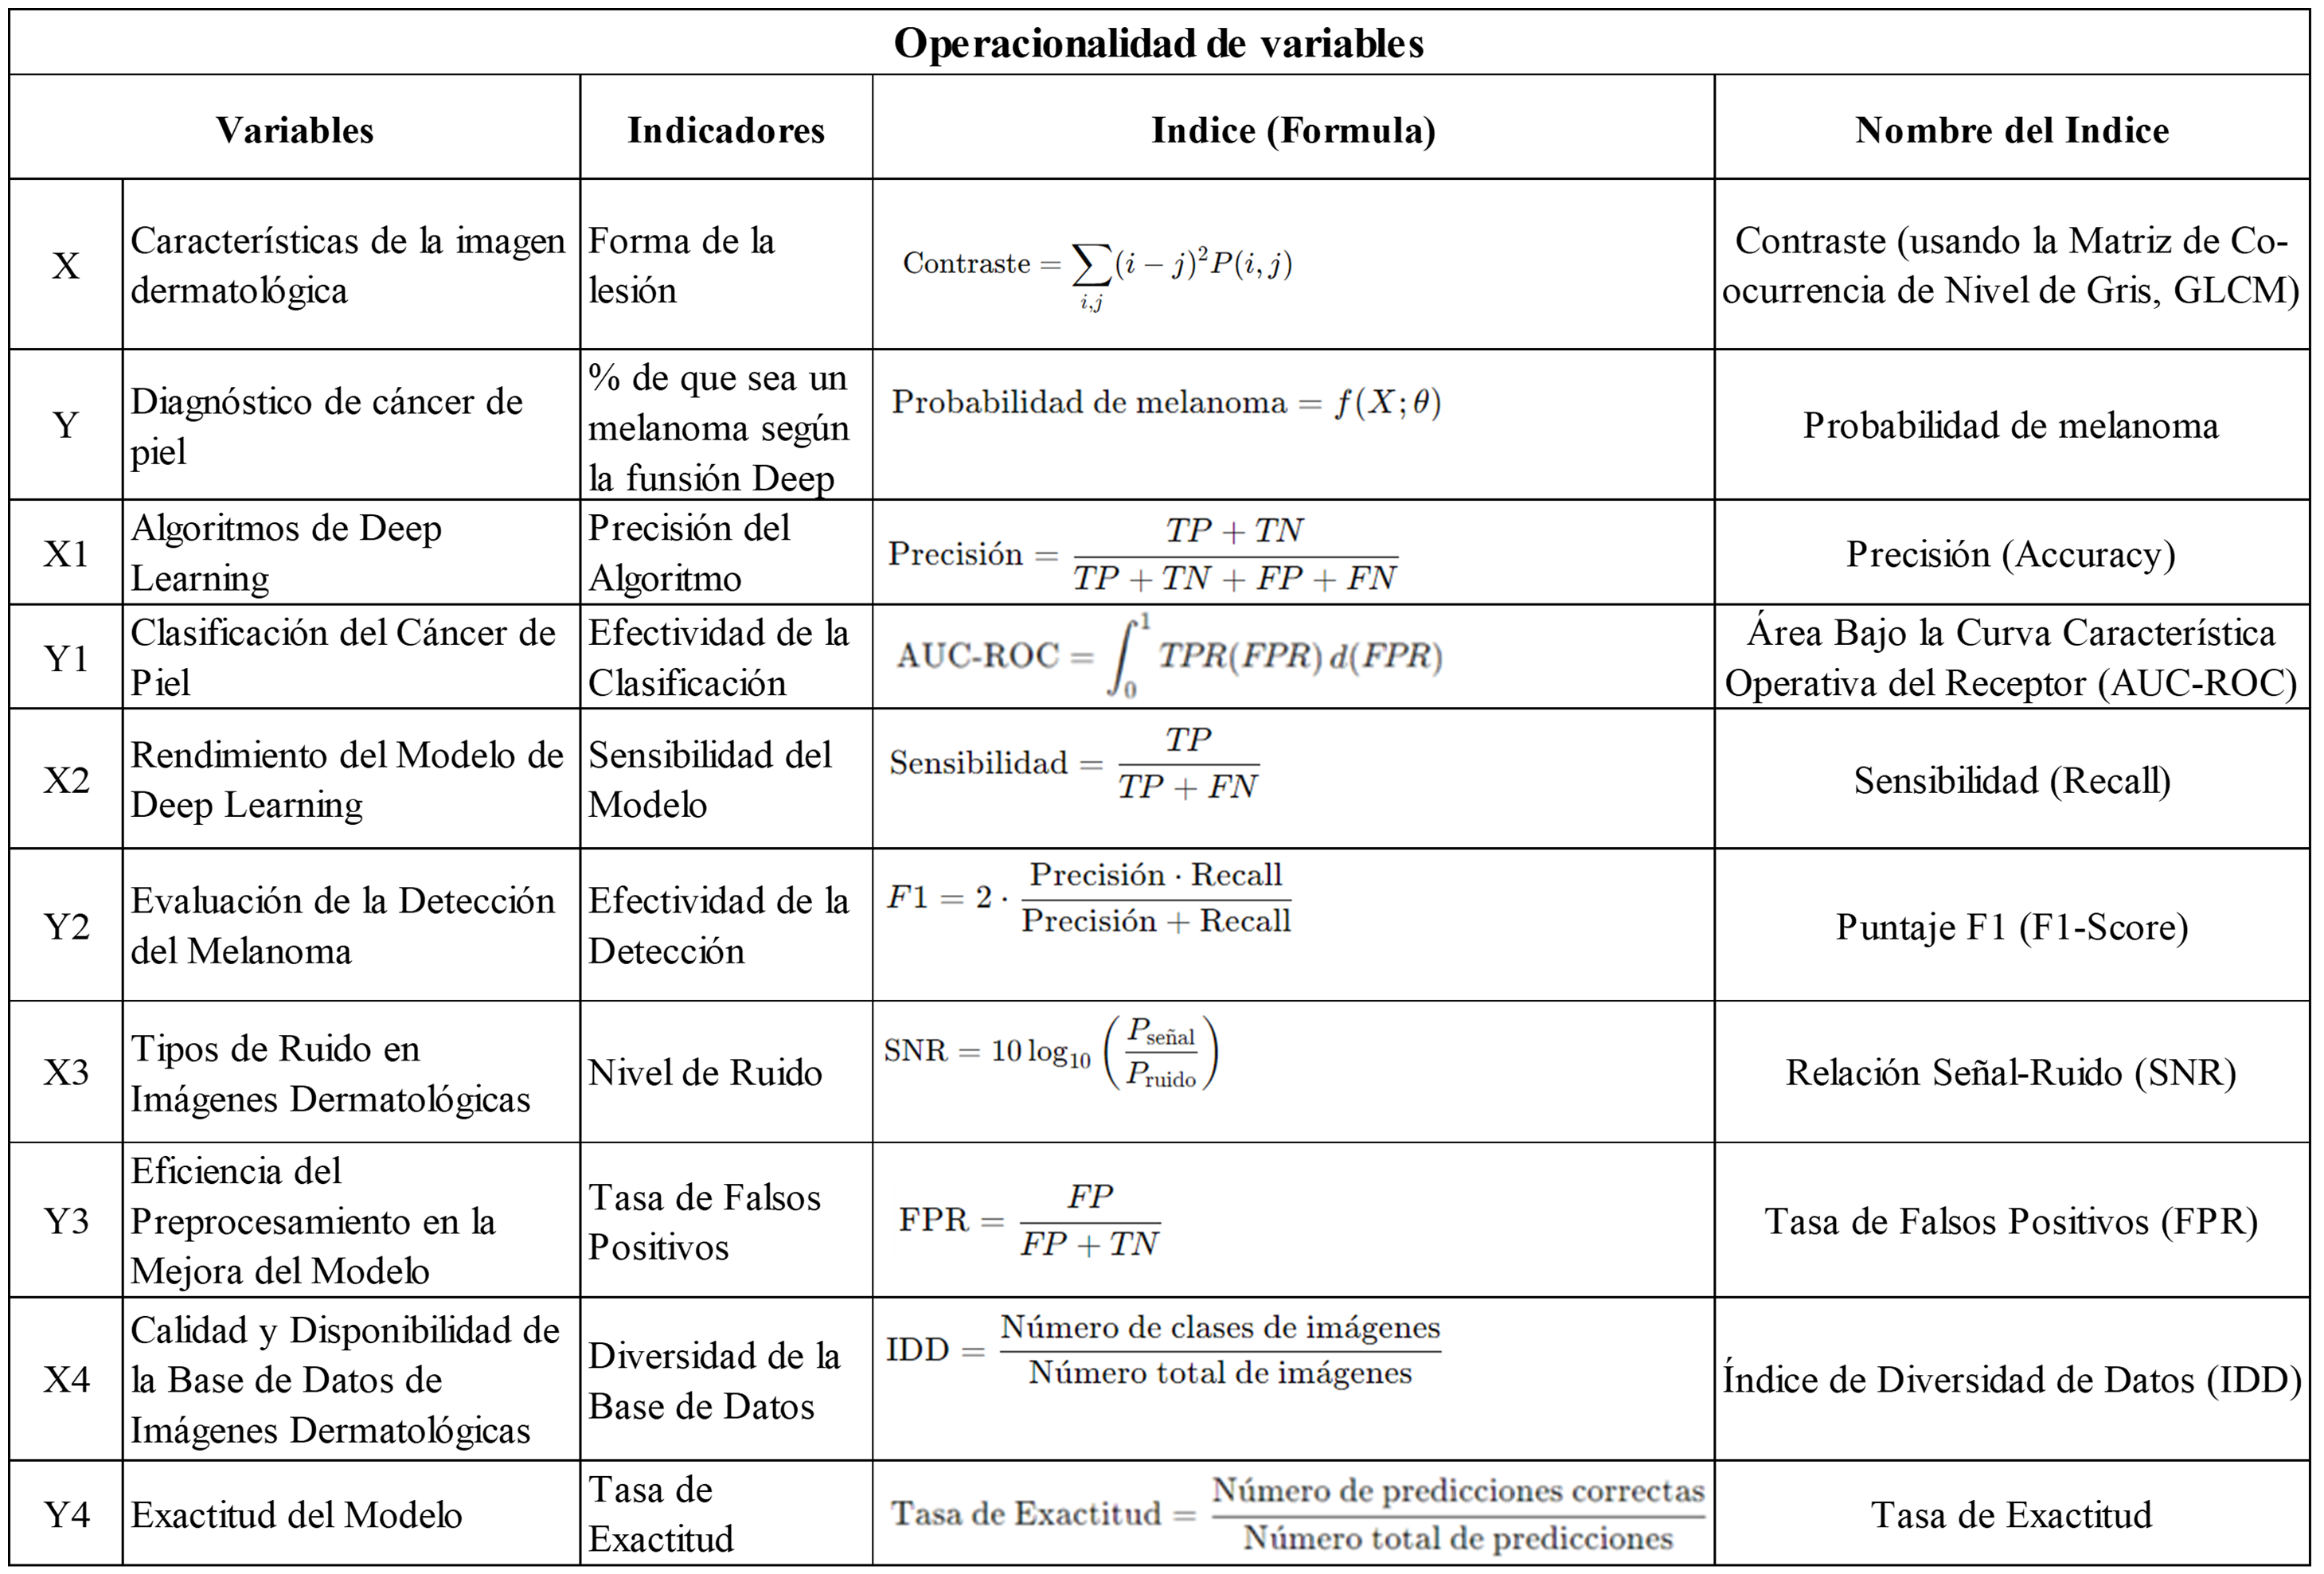
\includegraphics[width=0.9\textwidth]{3/figures/Operaciones de variables.png}
		\caption{Imagén de la Base de Datos. Fuente: Elaboracion propia}
		\label{1:fig 20}
	\end{center}
\end{figure}








\section{Técnicas de recolección}

Para el desarrollo de este trabajo tenemos 2 posibiles base de datos a usar.


1.-  Skin Cancer MNIST: HAM10000: Colección de múltiples imagenes dermatológicas del año 2018. Las variables se clasifican en tipos de lesión cutánea(melanoma/no melanoma). El tipo de análisis que se realizara es la clasificación y categorización las imágenes de acuerdo con los diferentes tipos de lesiones cutáneas.

\begin{figure}[h]
	\begin{center}
		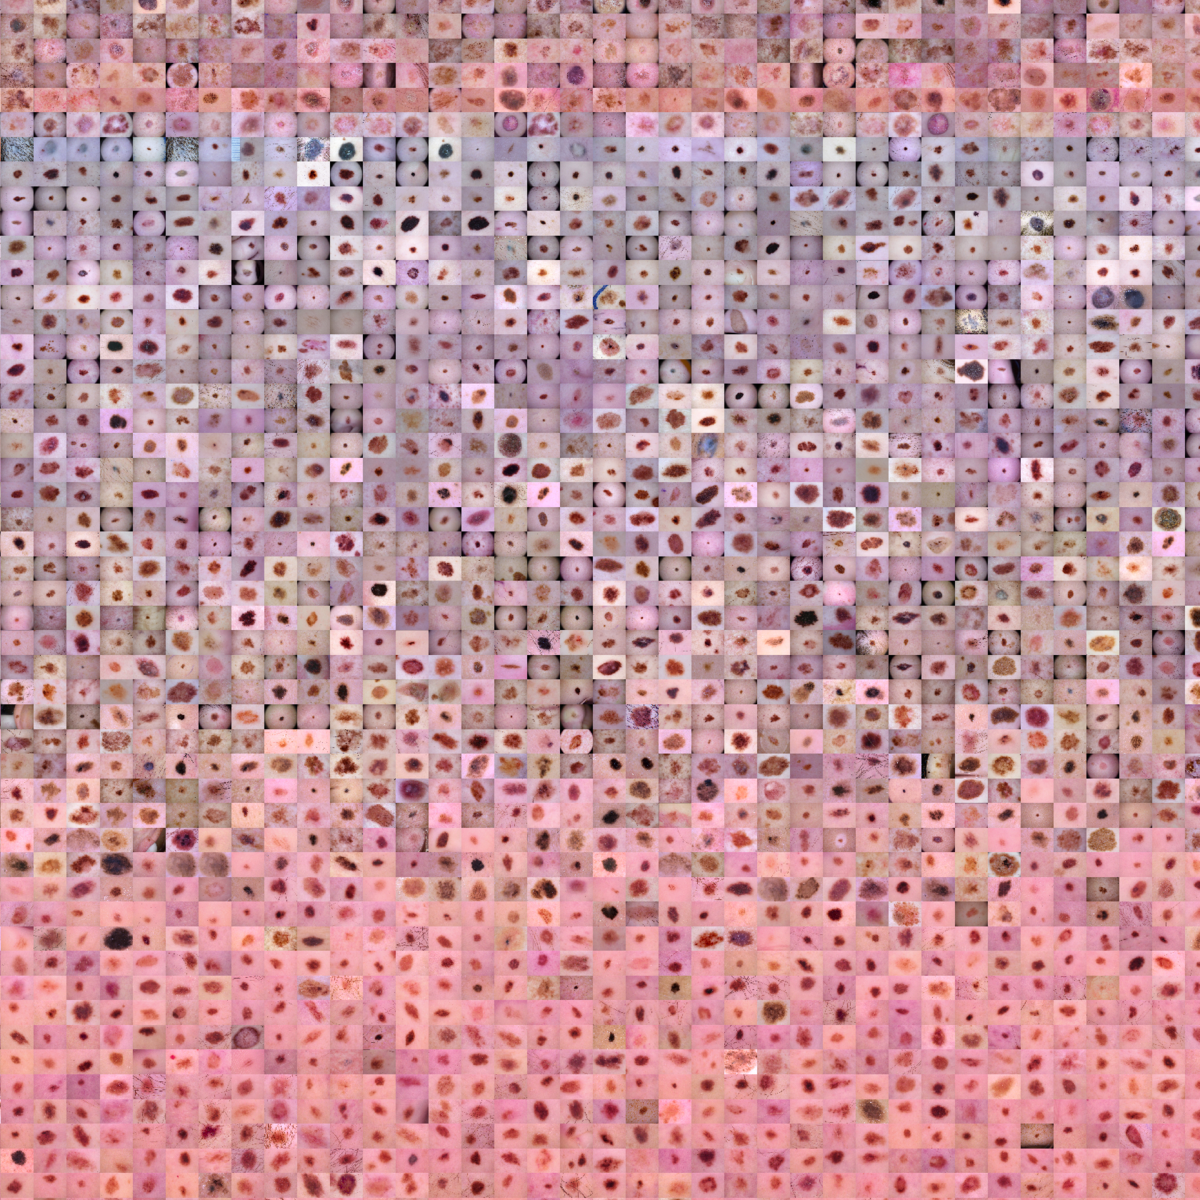
\includegraphics[width=0.25\textwidth]{3/figures/dataset-card.png}
		\caption{Imagen de la Base de Datos. Fuente: \cite{kaggleSkinCancer}}
		\label{1:fig 17}
	\end{center}
\end{figure}




\section{Técnicas para el procesamiento y análisis de la información}
Para escoger que metodología se usaria en el presente trabajo, se realizó un análisis de cada metodologías usada en los antecedentes presentados. No obstante, estos solo mencionan los pasos que realizaron para la implementacion de su investigacion.

 Aun así según la información recolectada se desidio implementar la metodología Iterativa. Esta por los siguentes puntos:
 
 - División del trabajo: Permite realizar una división según las partes del proyecto, facilitando la gestión y su seguimiento.
 
 - Adaptavilidad: Se le puede realizar ajustes si el proyecto lo requiere.
 
 Ahora se explicara los pasos a realizar en cada punto.
 


\subsection{Metodología de la implementación de la solución}



\begin{figure}[h]
	\begin{center}
		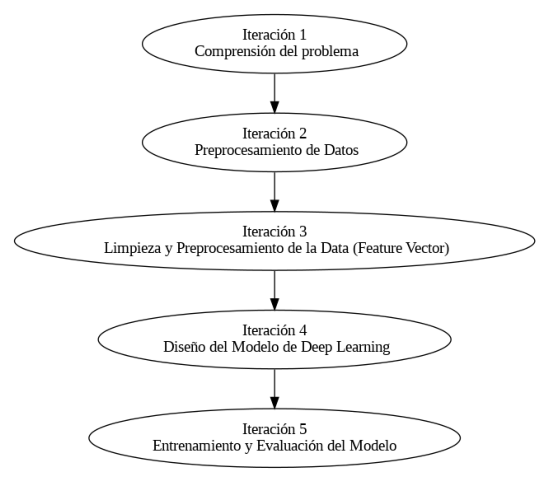
\includegraphics[width=0.5\textwidth]{3/figures/metodologia.png}
		\caption{Grafico de la Metodología a implementar. Fuente: Elavoración propia}
		\label{1:fig 19}
	\end{center}
\end{figure}


\newcommand{\MIPone}{Comprensión del problema: 
	Realizar una investigacion basica para la comprencion del tema a investigar. En este caso la detección temprana del melanoma es crucial para el tratamiento eficaz del cáncer de piel. No obstante, la evaluación manual de las imágenes cutáneas puede ser subjetiva y propensa a errores. Continuando, con la realizacion de una investigación de antecedente para determinar que tecnologia puede ayudar a automatizar y mejorar la precisión de deteccion del cander de melanoma.
	
}
\newcommand{\MIPtwo}{Descripción de la Base de datos: Se utilizará una base de datos de imágenes de lesiones cutáneas. Esta incluirá imágenes dermatoscópicas de melanomas y no melanomas.

Se revisara los antecedentes anterioes para ver que base de datos utilizaron. Si es posible usar usara una de esta o de lo contrario se indagara para la selección de otra.
Se dividida en conjuntos de entrenamiento, validación y prueba para evaluar el desempeño del modelo.
	
}
\newcommand{\MIPthree}{Limpieza y Preprocesamiento de Datos: 
	Se realizara la normalización del color, eliminación de artefactos, aumento de datos (data augmentation) y segmentación de las lesiones cutáneas. Se continuara con la implementacin de Feature Vectors para facilitar el aprendizaje del modelo en este caso haciendo uso de GLCM.  
	%% GLCM 
	
	
}
\newcommand{\MIPfour}{Diseño del Modelo de Deep Learning:
	Se realizara una arquitectura de redes neuronal profundas (DNN) y redes neuronales convolucionales (CNN) las cuales mediante averaging se promediara las predicciones de ambos modelos, mejorando el rendimiento general del sistema de clasificación.
	

}
\newcommand{\MIPfive}{Entrenamiento y Evaluación del Modelo: El modelo se entrenará utilizando el conjunto de datos de entrenamiento, ajustando los hiperparámetros para optimizar su desempeño. El modelo será evaluado en el conjunto de validación y prueba, utilizando métricas como la precisión, sensibilidad, especificidad, y la curva ROC-AUC para medir su efectividad en la detección del melanoma.
	
}




\begin{itemize}
	\item \MIPone
	\item \MIPtwo
	\item \MIPthree
	\item \MIPfour
	\item \MIPfive
	%\item \MIPsix
	
\end{itemize}

	






\subsubsection{Metodología para la medición de resultados}

Para evaluar la performance de un modelo, se utilizan diversas métricas como instrumentos de medición de desempeño a partir de los resultados arrojados en la Matriz de confusión. A continuación, se detalla su concepto y sus elementos.


%La fórmula de Precisión (Accuracy) se define como:
 
%\begin{equation}
%	\text{Precisión} = \frac{TP + TN}{TP + TN + FP + FN}
%\end{equation}

%Esta formula sera usada para la precisio del algoritmo.


%% formula 1
La fórmula de Área Bajo la Curva Característica Operativa del Receptor (AUC-ROC) se define como:
\begin{equation}
	\text{AUC-ROC} = \int_{0}^{1} TPR(FPR) \, d(FPR)
\end{equation}

Esta formula sera usada para la efectividad de la Clasificación





%% formula 2
La fórmula Puntaje F1 (F1-Score) se define como:

\begin{equation}
	F1 = 2 \cdot \frac{\text{Precisión} \cdot \text{Recall}}{\text{Precisión} + \text{Recall}}
\end{equation}
Esta formula sera usada fectividad de la Detección




%% formula 3
La fórmula de Tasa de Falsos Positivos se define como:

\begin{equation}
	\text{FPR} = \frac{FP}{FP + TN}
\end{equation}
Esta formula sera usada para evaluar la eficiencia del preprocesamiento en la mejora del modelo




%% formula 4
La fórmula de exactitud del Modelo se define como:
\begin{equation}
	\text{Tasa de Exactitud} = \frac{\text{Número de predicciones correctas}}{\text{Número total de predicciones}}
\end{equation}

Esta formula sera usada para evaluar exactitud del modelo





\section{Cronograma de actividades}

Se elaboró un cronograma de actividades de toda la investigación, mostrada en la Figura \ref{3:fig13}, contemplando desde el inicio del año 2024 hasta finales del 2024, donde se realizara la sustentacion del trabajo.

\begin{figure}[h]
	\begin{center}
		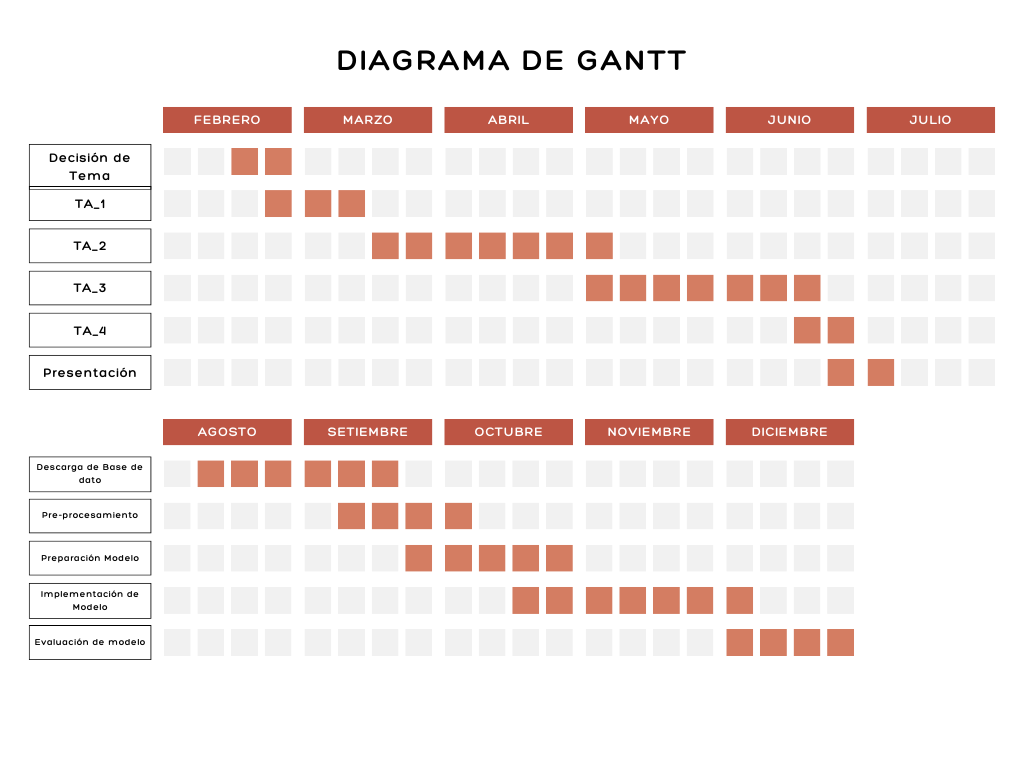
\includegraphics[width=1\textwidth]{3/figures/Cronograma Diagrama de Gantt.png}
		\caption{Diagrama de Grantt. Fuente: Elavoración Propia }
		\label{1:fig 18}
	\end{center}
\end{figure}




\section{Presupuesto}

\begin{center}
	\begin{tabular}{|p{8cm}|p{3cm}|}
		\hline
		Materiales & Costos  \\
		\hline
		Computadora Core i7 & 2000 \\
		\hline

		Total & 2000 \\
		\hline
	\end{tabular}
\end{center}


\begin{comment}
\begin{table}[h!]
	\centering
	\begin{tabular}{|l|p{10cm}|}
		\hline
		\textbf{Concepto} & \textbf{Descripción} \\ \hline
		Población & Personas con lesiones cutáneas, específicamente aquellas que presentan diferentes tipos de cáncer de piel y otras afecciones dermatológicas. \\ \hline
		Muestra & El conjunto de datos contiene un total de 10,015 imágenes de dermatoscopia de lesiones cutáneas. \\ \hline
		Unidad de análisis & Cada imagen de dermatoscopia es una unidad de análisis. Estas imágenes representan diferentes tipos de lesiones cutáneas. \\ \hline
		Variable y tipo de análisis & Clase de la lesión cutánea (melanoma/no melanoma). Clasificación y categorización de las imágenes de acuerdo a los diferentes tipos de lesiones cutáneas. \\ \hline
	\end{tabular}
	
	\label{tabla:dataset}
\end{table}
\end{comment}


\begin{comment}

 Nisi porta lorem mollis aliquam ut porttitor leo. Aenean pharetra magna ac placerat vestibulum. Est placerat in egestas erat imperdiet sed euismod. Velit euismod in pellentesque massa placerat. Enim praesent elementum facilisis leo vel fringilla. Ante in nibh mauris cursus mattis molestie a iaculis. Erat pellentesque adipiscing commodo elit at imperdiet dui accumsan sit. Porttitor lacus luctus accumsan tortor posuere ac ut. Tortor at auctor urna nunc id. A iaculis at erat pellentesque adipiscing commodo elit. La Figura \ref{fig1} y el Cuadro \ref{tab:widgets}

	\begin{figure}[h]
		\begin{center}
			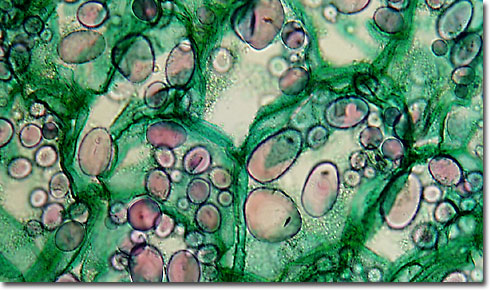
\includegraphics[width=0.8\textwidth]{3/figures/largepotato.jpg}
			\caption{Prueba de Figura}
			\label{fig1}
		\end{center}
		
	\end{figure}


\section{Operacionalización de Variables}

Nisi porta lorem mollis aliquam ut porttitor leo. Aenean pharetra magna ac placerat vestibulum. Est placerat in egestas erat imperdiet sed euismod. Velit euismod in pellentesque massa placerat. Enim praesent elementum facilisis leo vel fringilla. Ante in nibh mauris cursus mattis molestie a iaculis. Erat pellentesque adipiscing commodo elit at imperdiet dui accumsan sit. Porttitor lacus luctus accumsan tortor posuere ac ut. Tortor at auctor urna nunc id. A iaculis at erat pellentesque adipiscing commodo elit.
\section{Instrumentos de medida}
Nisi porta lorem mollis aliquam ut porttitor leo. Aenean pharetra magna ac placerat \begin{itemize}
	\item muscle and fat cells remove glucose from the blood,
	\item cells breakdown glucose via glycolysis and the citrate cycle, storing its energy in the form of ATP,
	\item liver and muscle store glucose as glycogen as a short-term energy reserve,
	\item adipose tissue stores glucose as fat for long-term energy reserve, and
	\item cells use glucose for protein synthesis.
\end{itemize}

\section{Técnicas de recolección de datos}
Nisi porta lorem mollis aliquam ut porttitor leo. Aenean pharetra magna ac placerat vestibulum. Est placerat in egestas erat imperdiet sed euismod. Velit euismod in pellentesque massa placerat. Enim praesent elementum facilisis leo vel fringilla. Ante in nibh mauris cursus mattis molestie a iaculis. Erat pellentesque adipiscing commodo elit at imperdiet dui accumsan sit. Porttitor lacus luctus accumsan tortor posuere ac ut. Tortor at auctor urna nunc id. A iaculis at erat pellentesque adipiscing commodo elit.

\LaTeX{} is great at typesetting mathematics. Let $X_1, X_2, \ldots, X_n$ be a sequence of independent and identically distributed random variables with
\begin{equation}
	S_n = \frac{X_1 + X_2 + \cdots + X_n}{n}
	= \frac{1}{n}\sum_{i}^{n} X_i
	\label{eq1}
\end{equation}

La Ecuación \ref{eq1} denote their mean. Then as $n$ approaches infinity, the random variables $$\sqrt{n}(S_n - \mu)$$ converge in distribution to a normal $\mathcal{N}(0, \sigma^2)$.

\section{Técnicas para el procesamiento y análisis de la información}
Nisi porta lorem mollis aliquam ut porttitor leo. Aenean pharetra magna ac placerat vestibulum. Est placerat in egestas erat imperdiet sed euismod. Velit euismod in pellentesque massa placerat. Enim praesent elementum facilisis leo vel fringilla. Ante in nibh mauris cursus mattis molestie a iaculis. Erat pellentesque adipiscing commodo elit at imperdiet dui accumsan sit. Porttitor lacus luctus accumsan tortor posuere ac ut. Tortor at auctor urna nunc id. A iaculis at erat pellentesque adipiscing commodo elit.

You can make lists with automatic numbering \dots

\begin{enumerate}
	\item Like this,
	\item and like this.
\end{enumerate}
\dots or bullet points \dots
\begin{itemize}
	\item Like this,
	\item and like this.
\end{itemize}


\section{Cronograma de actividades y presupuesto}
Nisi porta lorem mollis aliquam ut porttitor leo. Aenean pharetra magna ac placerat vestibulum. Est placerat in egestas erat imperdiet sed euismod. Velit euismod in pellentesque massa placerat. Enim praesent elementum facilisis leo vel fringilla. Ante in nibh mauris cursus mattis molestie a iaculis. Erat pellentesque adipiscing commodo elit at imperdiet dui accumsan sit. Porttitor lacus luctus accumsan tortor posuere ac ut. Tortor at auctor urna nunc id. A iaculis at erat pellentesque adipiscing commodo elit.

\begin{table}[h]
	\centering
	\begin{tabular}{l|r}
		Item & Quantity \\\hline
		Widgets & 42 \\
		Gadgets & 13
	\end{tabular}
	\caption{\label{tab:widgets}An example table.}
\end{table}

\end{comment}

